\subsection{MMLU (Massive Multitask Language Understanding)}
{{\footnotesize
\noindent Measuring Massive Multitask Language Understanding (MMLU) is a benchmark of 57 
multiple-choice tasks covering elementary mathematics, US history, computer science, 
law, and more, designed to evaluate a model's breadth and depth of knowledge in 
zero-shot and few-shot settings.


\begin{description}[labelwidth=4cm, labelsep=1em, leftmargin=4cm, itemsep=0.1em, parsep=0em]
  \item[date:] 2020-09-07
  \item[version:] 1
  \item[last\_updated:] 2020-09-07
  \item[expired:] false
  \item[valid:] yes
  \item[valid\_date:] 2025-07-28
  \item[url:] \href{https://paperswithcode.com/dataset/mmlu}{https://paperswithcode.com/dataset/mmlu}
  \item[doi:] 10.48550/arXiv.2009.03300
  \item[domain:] Multidomain
  \item[focus:] Academic knowledge and reasoning across 57 subjects
  \item[keywords:]
    - multitask
    - multiple-choice
    - zero-shot
    - few-shot
    - knowledge probing
  \item[licensing:] MIT License
  \item[task\_types:]
    - Multiple choice
  \item[ai\_capability\_measured:]
    - General reasoning, subject-matter understanding
  \item[metrics:]
    - Accuracy
  \item[models:]
    - GPT-4o
    - Gemini 1.5 Pro
    - o1
    - DeepSeek-R1
  \item[ml\_motif:]
    - General knowledge
  \item[type:] Benchmark
  \item[ml\_task:]
    - Supervised Learning
  \item[solutions:] 1
  \item[notes:] Good
  \item[contact.name:] Dan Hendrycks
  \item[contact.email:] dan (at) safe.ai
  \item[datasets.links.name:] Papers with Code datasets
  \item[datasets.links.url:] \href{https://github.com/paperswithcode/paperswithcode-data}{https://github.com/paperswithcode/paperswithcode-data}
  \item[results.links.name:] Chinchilla
  \item[results.links.url:] \href{https://arxiv.org/abs/2203.15556}{https://arxiv.org/abs/2203.15556}
  \item[fair.reproducible:] True
  \item[fair.benchmark\_ready:] True
  \item[id:] mmlu\_massive\_multitask\_language\_understanding
  \item[Citations:] \cite{hendrycks2021measuring}
\end{description}

{\bf Ratings:} ~ \\

\begin{tabular}{p{0.15\textwidth} p{0.07\textwidth} p{0.7\textwidth}}
\hline
Rating & Value & Reason \\
\hline
dataset & 5 & Meets all FAIR principles and properly versioned.
 \\
documentation & 5 & Well-explained in a provided paper.
 \\
metrics & 5 & Fully defined, represents a solution's performance.
 \\
reference\_solution & 2 & Reference models are available (i.e. GPT-3), but are not trainable or publicly documented
 \\
software & 0 & No instructions to download or run data given on the site
 \\
specification & 4 & No system constraints
 \\
\hline
\end{tabular}

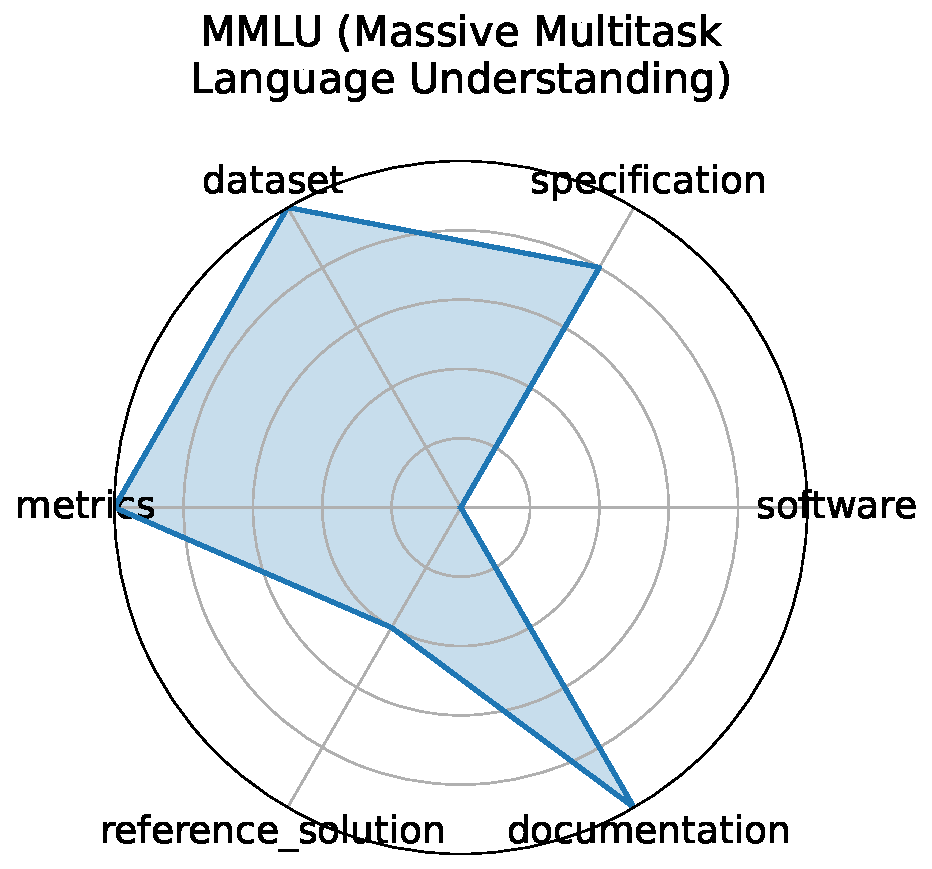
\includegraphics[width=0.2\textwidth]{mmlu_massive_multitask_language_understanding_radar.pdf}
}}
\clearpage